\frame{
    \frametitle{The learning rate}
    \begin{block}{Neighborhood function $\Theta$: the learning rate $\alpha$}
        \begin{equation*}
            \alpha(t)\cdot\Theta(t,\beta_{1},\beta_{2})
        \end{equation*}
        \begin{columns}
            \begin{column}{0.4\textwidth}
                $\sigma = 1.7$, $\alpha=0.5$\\
                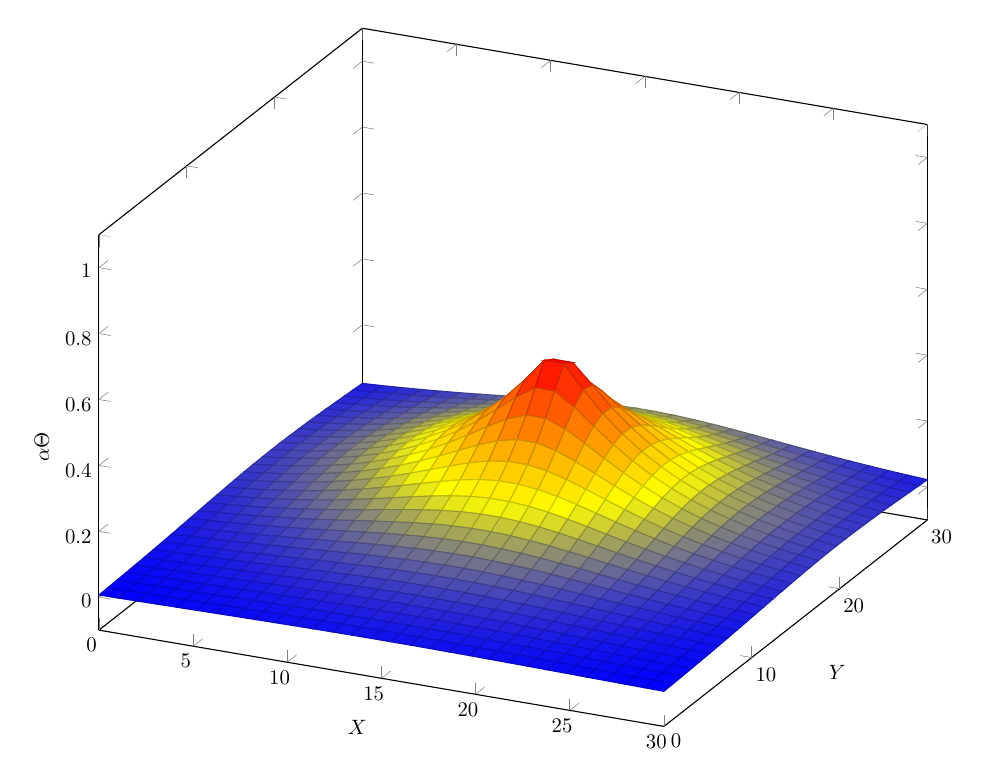
\begin{tikzpicture}[scale=1, every node/.style={scale=0.75}]
                    \pgfplotsset{width=\textwidth,compat=1.3}
                          \begin{axis}[xlabel=$X$, ylabel=$Y$,zlabel=$\alpha\Theta$]
                          \addplot3[surf,shader=faceted,domain=0:30, samples=30]
                              {0.5*(exp( -1 * ( sqrt((x-15)^2+(y-20)^2)/(2*1.7^2) ) ))};
                    \addplot3[color=black, mark=none] plot coordinates {(0,0,0) (0,0,1)};
                         \end{axis}
                \end{tikzpicture}
            \end{column}
            \begin{column}{0.4\textwidth}
                $\sigma=1$, $\alpha=0.25$\\
                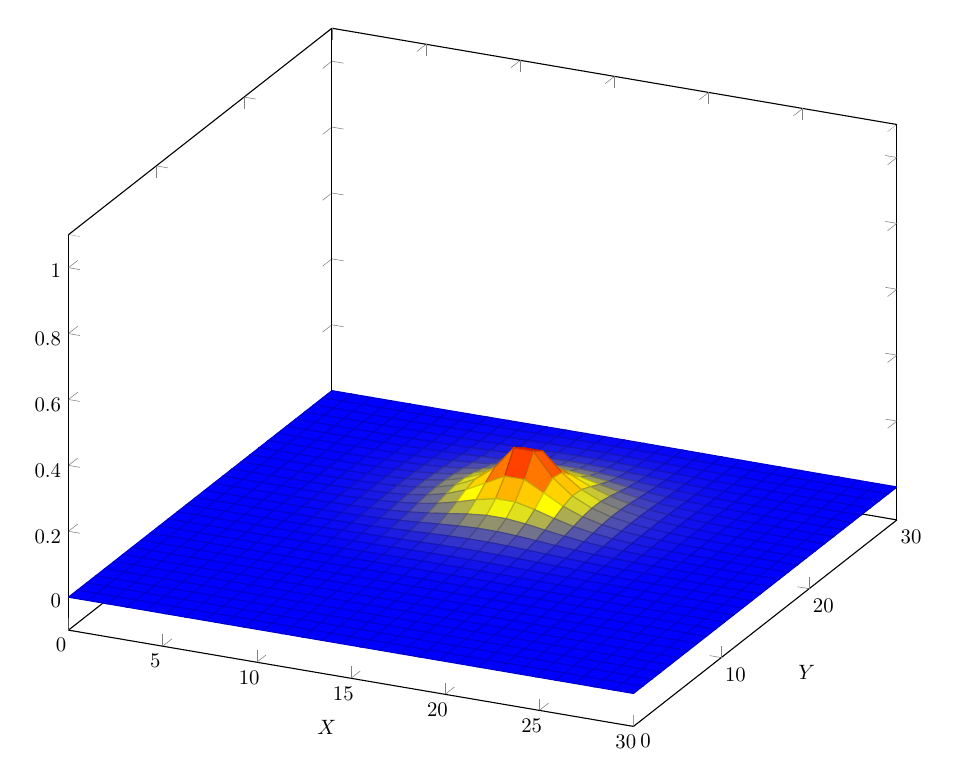
\begin{tikzpicture}[scale=1, every node/.style={scale=0.75}]
                    \pgfplotsset{width=\textwidth,compat=1.3}
                          \begin{axis}[xlabel=$X$, ylabel=$Y$]
                          \addplot3[surf,shader=faceted,domain=0:30, samples=30]
                              {0.25*(exp( -1 * ( sqrt((x-15)^2+(y-20)^2)/(2*1^2) ) ))};
                    \addplot3[color=black, mark=none] plot coordinates {(0,0,0) (0,0,1)};
                         \end{axis}
                \end{tikzpicture}
            \end{column}
        \end{columns}
        \begin{equation*}
        \alpha(t)=(\alpha(t_{i})-\alpha(t_{f}))\cdot\exp(-\frac{t}{\lambda})+\alpha(t_{f})
        \end{equation*}
    \end{block}
}
